%%%%%%%%%%%%%%%%%%%%%%%%%%%%%%%%%%%%%%%%%%%%%%%%%%%%%%%%%%%%%%%%%%%%%%%%
% Plantilla TFG/TFM
% Escuela Politécnica Superior de la Universidad de Alicante
% Realizado por: Jose Manuel Requena Plens
% Contacto: info@jmrplens.com / Telegram:@jmrplens
%%%%%%%%%%%%%%%%%%%%%%%%%%%%%%%%%%%%%%%%%%%%%%%%%%%%%%%%%%%%%%%%%%%%%%%%

\chapter{Metodología y Planificación}

En el desarrollo de este trabajo fue necesario definir una metodología clara que sirviera de guía a lo largo de todo el proceso. El proyecto presentaba una dificultad añadida frente a otros trabajos puramente software: la necesidad de establecer conectividad con routers Cisco en un entorno de simulación mediante GNS3. Este aspectó condicionó desde el inicio la planificaación, ya que sin resolver esta problemática no era posible avanzar hacia fases posteriores. Por este movito, la consecución de la conectividad se planteó como el primer objetivo fundamental dentro de la metodología adoptada.

Una vez superado este hito, el trabajo se organizó de manera secuencial. En primer lugar, se implementó el backend, encargado de gestionar la comunicación con los routers y el tratamiento de la información obtenida. Posteriormente, se desarrolló el frontend, con el propósito de representar los datos de manera visual e intuitiva. Todo el proceso se llevó a cabo siguiendo un enfoque iterativo, en el que cada avance era probado y validado antes de pasar al siguiente, lo que permitió corregir errores de forma temprana y ajustar la planificación conforme se identificaban nuevas necesidades.

\section{Metodología de trabajo}

Para el siguiente proyecto se optó por una metodología de carácter iterativo e incremental, adaptada a las necesidades concretas del trabajo. La elección de este enfoque respondió a la naturaleza experimental del sistema planteado, en el que era previsible encontrar dificultades técnicas relacionadas principalmente con la conectividad a los routers y la extracción de información en tiempo real. Adptar un modelo rígido de desarrollo (como el modelo en cascada) habría limitado la capacidad de reacción ante imprevistos, por lo que se consideró más adecuado trabajar con ciclos cortos de análisis, implementación y validación. Para la estructura de la metodología se siguió el diagrama de fases representado en la Figura~\ref{fig:fases},

\begin{figure}[H]
    \centering
    {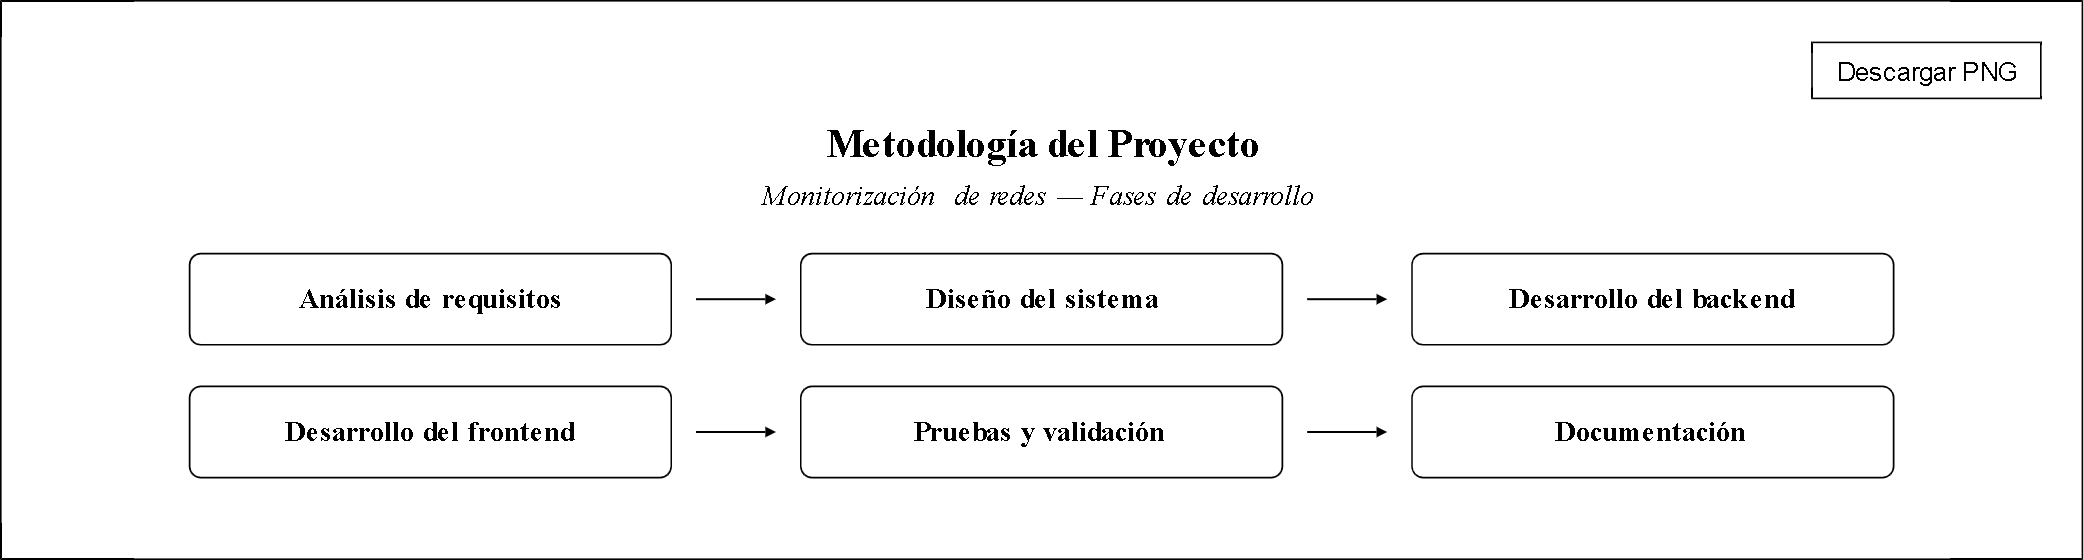
\includegraphics[width=0.95\linewidth]{imagenes/image15.png}}
    \caption{Diagrama de fases}
    \label{fig:fases}
\end{figure}

El proyecto se estructuró en fases principales, cada una de las cuales finalizaba con un resultado verificable antes de pasar a la siguiente. En primer lugar, se realizó el análisis de requisitos, en el que identificaron la funcionalidades necesarias (obtención d estadísticas de tráfico, estado de interfaces, uso de CPU, detección de errores, entre otras) y las limitaciones técnicas del entorno de trabajo. La segunda fase correspondió al diseño de la arquitectura, en la que se definió la división entre el backend y el frontend, así como la forma de interactuar con los routers a través de conexiones SSH.

A continuación, se llevó a cabo la fase de implementación, que se organizó de manera incremental. En esta etapa, la prioridad inicial fue conseguir la conectvidad estable con los routers y extraer información básica de la interfaces. Una vez validado este punto, se desarrollaron los módulos principales del backend con FastAPI, encargados de procesar y servir los datos del sistema. Posteriormente, se diseñó el frontend con Vue.js y Bootsrap, orientado a la visualización clara e interactiva de la información obtenida.

La metodología adoptada también completó un proceso de pruebas continuas. Cada módulo desarrollado se validaba en escenarios de red emulados en GNS3, lo que permitió detectar errores en fases tempranas y garantizar que los comopnentes eran funcionales antes de integrarlos con el resto del sistema. Además las revisiones periódicas con el tutor del proyecto facilitaron la reorientación de tareas cuando surgían dificultades, manteniendo el trabajo alineado con los objetivos planteados.



\section{Herramientas utilizadas}
\section{Planificación temporal}
\section{Herramientas de gestión}


